%%mark = star, diamond, square, otimes
%\documentclass{article}
%\usepackage{pgfplots}
%\usepackage[justification=centering]{caption}
%\pgfplotsset{compat=newest}
%\begin{document}
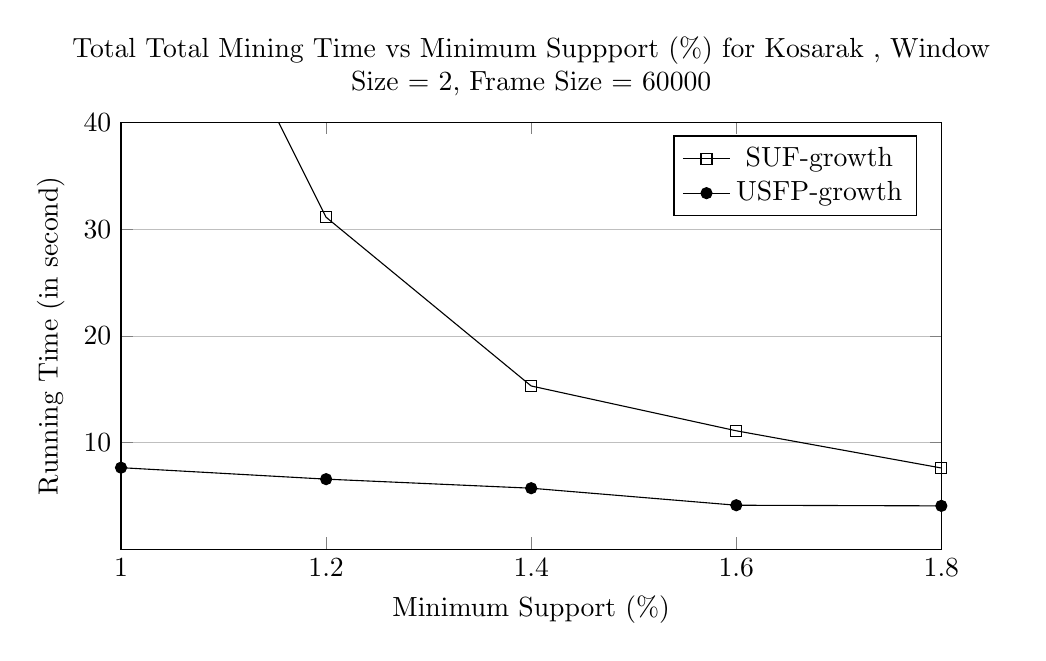
\begin{tikzpicture}
\begin{axis}[
	title={\parbox{\linewidth}{\centering Total Total Mining Time vs Minimum Suppport (\%) for Kosarak , Window Size = 2, Frame Size = 60000}},
	width=12cm,
	height=7cm,
    xlabel={Minimum Support (\%) },
    ylabel={Running Time (in second)},
    xmin=1.0, xmax=1.8,
    ymin=0, ymax=40,
    xtick={1.0,1.2,1.4,1.6,1.8},
    ytick={10,20,30,40},
    legend pos=north east,
    ymajorgrids=true,
    grid style={line width=.2pt,draw=gray!50},
]
 
\addplot[
    solid, every mark/.append style={solid, fill=gray}, mark=square
    ]
    coordinates {
		(1.0  ,	69.55)
		(1.2,	31.13)
		(1.4,	15.310)
		(1.6,	11.108)
		(1.8,	7.620)
};
    \addlegendentry{SUF-growth}
\addplot[
    solid, every mark/.append style={solid, fill=black}, mark=*
    ]
    coordinates {
		(1.0 ,	7.650	)
		(1.2,	6.575	)
		(1.4,	5.725	)
		(1.6,	4.128	)
		(1.8,	4.069	)
};
    \addlegendentry{USFP-growth}
 
\end{axis}
\end{tikzpicture}
%\end{document}